\documentclass[11pt,letterpaper]{article}
\usepackage[margin=1in]{geometry}
\usepackage[T1]{fontenc}
\usepackage{lmodern,amsmath,amssymb,booktabs,graphicx,enumitem,microtype,xurl}
\usepackage[hidelinks]{hyperref}
\usepackage{fancyhdr}
\pagestyle{fancy}\fancyhf{}\fancyhead[L]{Traceable entity reconciliation}\fancyhead[R]{Detailed research manuscript}\fancyfoot[C]{\thepage}
\setlength{\headheight}{14pt}
\setlength{\parskip}{4pt}
\setlength{\emergencystretch}{2em}
\setlist{nosep}
\newcommand{\FWwiAttr}{0.7688}
\newcommand{\FWwiGraph}{0.7888}
\newcommand{\FWwiAug}{0.7626}
\newcommand{\FOlistAttr}{0.6919}
\newcommand{\FOlistGraph}{0.7842}
\newcommand{\FOlistAug}{0.7414}
\newcommand{\FDataCoAttr}{0.6962}
\newcommand{\FDataCoGraph}{0.6750}
\newcommand{\FDataCoAug}{0.6962}
\newcommand{\FBpiAttr}{0.1242}
\newcommand{\FBpiGraph}{0.5734}
\newcommand{\FBpiAug}{0.1492}
\newcommand{\WdcAttr}{0.5369}
\newcommand{\WdcAug}{0.5584}
\newcommand{\WdcEmb}{0.3919}

\newcommand{\tabsource}{\par\smallskip\textit{Source: verified all-datasets-v1 artifacts; generated values.}}
\title{Traceable Entity Reconciliation with Gated Transaction Context:\\A Five-Dataset Evaluation of Fidelity, Matching, Queries, Robustness, and Scale}
\author{Anonymous research draft}
\date{October 12, 2026}
\begin{document}
\maketitle
\begin{abstract}
Cross-system entity reconciliation affects both record matching and the answers obtained from integrated enterprise data. This paper presents an auditable prototype that preserves typed source relationships and provenance, combines attribute evidence with gated transaction context, and materializes constrained identity decisions without replacing source records. Five linked evaluations examine import fidelity, matching, downstream query accuracy, robustness and calibration, and computational scaling. The exploratory study uses Wide World Importers (WWI), Olist, DataCo, BPI Challenge 2019, and all 27 official pairwise WDC Products configurations, with three seeds and no human study. On common ambiguous candidates, mean F1 changes from \FWwiAttr{} to \FWwiGraph{} on WWI, from \FOlistAttr{} to \FOlistGraph{} on Olist, from \FDataCoAttr{} to \FDataCoGraph{} on DataCo, and from \FBpiAttr{} to \FBpiGraph{} on BPI. The BPI baseline uses coarse history descriptors rather than vendor names. Flat SQL and graph extraction produce the same context scores, isolating evidence from representation. WDC has no transaction graph; a frozen embedding feature raises fully unseen mean F1 from \WdcAttr{} to \WdcAug{}. Eighteen official WDC configurations have development-test offer overlaps and are flagged. All applicable query controls preserve SQL/graph answer equality, while predicted identities leave task-specific errors. Forty-five scaling trials expose substantial candidate-recall losses under output caps and replicated workloads. The evidence supports traceable integration and conditional contextual benefit, with a negative DataCo result; it does not establish universal accuracy gains, graph-specific predictive superiority, production scalability, or human usefulness.
\end{abstract}
\noindent\textbf{Keywords:} entity resolution; knowledge graphs; transaction context; provenance; reproducible evaluation.

\section{Introduction}
Enterprise data integration requires more than collecting records into a common store. Purchasing, warehouse, finance, e-commerce and process systems may assign different identifiers to observations of the same customer, supplier or product. A join that depends on unresolved identity can omit valid transactions. An incorrect merge can attach transactions to the wrong entity and produce plausible but incorrect aggregates. Reconciliation is therefore both a statistical task and a data-management decision whose consequences should be inspectable.

Attribute similarity supplies a useful initial signal. Names, categories, units and descriptive text can agree even when local identifiers differ. However, descriptive fields may be abbreviated, absent, shared by multiple entities or unsuitable for comparison. Transaction histories offer additional observations: products bought, activities performed, categories visited, timing and compatible quantities. These observations can also be sparse, misleading or correlated with already visible attributes. Simply adding a graph representation cannot establish that its relationships add information, nor that a higher pairwise F1 improves a particular query.

We study a conservative implementation in which source records remain intact, candidate scoring excludes evaluator identity, and context is used only when an adapter-specific support test passes. Accepted links form an auditable canonical view under type and one-to-one constraints. The evaluated artifact uses an in-memory property graph for matching projections and a disk-backed typed graph for large source imports. It is a prototype rather than a deployed ERP integration platform.

The contribution is an integrated evaluation design and its implemented controls. First, native foreign-key reference sets test whether graph construction preserves source relationships. Second, common candidates and a shared learner catalog isolate the contribution of permitted context within each task. Third, independent flat SQL extraction tests whether the same evidence yields the same features and scores. Fourth, query evaluation separates representation agreement from identity correctness. Fifth, perturbations, calibration audits and three-point scaling reveal where support, thresholds and retrieval fail. These controls are useful precisely because some measured results are negative or qualified.

The study began with WWI and WDC as primary datasets and then expanded to Olist, DataCo and BPI. The expanded run is exploratory: a source adapter was revised after examining context availability, and query/provenance implementations were corrected with saved amendments. Original results and the original short manuscript are preserved. The present paper integrates the completed expanded evidence without recasting that development history as preregistration.

The research questions are: \textbf{RQ1}, does typed ingestion preserve in-scope source records, relationships and lineage? \textbf{RQ2}, does permitted gated context improve matching over attributes on the same candidates? \textbf{RQ3}, how do identity decisions affect source-level query answers, and do SQL and graph implementations agree? \textbf{RQ4}, how do defects and support removal affect matching and decision reliability? \textbf{RQ5}, what computational and retrieval trade-offs arise as projected workloads grow? Each question has a corresponding experiment, E1--E5. Human evaluation is outside the study.

\section{Related Work and Research Position}
Relational information is established evidence for entity resolution. Bhattacharya and Getoor describe collective resolution in which relationships between references participate in disambiguation~\cite{collective}. GraphER combines graph differential dependencies with neural graph processing~\cite{grapher}. Our artifact does not reproduce either approach. It uses explicit summaries and a support gate, enabling evidence inspection and a flat-relational parity control. Its novelty claim concerns this evaluated integration of controls, not the general idea of relational entity resolution.

Pretrained language models provide another established route to matching. Ditto fine-tunes a pair classifier using pretrained language models and task-specific processing~\cite{ditto}. Sentence-BERT provides sentence representations for similarity comparison~\cite{sbert}, and MiniLM studies transformer compression through distillation~\cite{minilm}. Here the executable neural reference is a frozen, quantized all-MiniLM-L6-v2 encoder~\cite{modelcard}. Only its scalar pair cosine is supplied to the common learner catalog. Results cannot be interpreted as comparisons against a reproduced Ditto system, a trained GNN or an optimized transformer matcher.

Blocking and filtering reduce the candidate search space, but their recall constrains the downstream system~\cite{blocking}. We report both candidate-conditioned accuracy and full-positive-universe accuracy. At scale, we also distinguish the imposed bound on emitted pairs from the internal work needed to retrieve and rank them. This distinction prevents a candidate-count trend from being presented as a complexity theorem.

WDC Products organizes evaluation around corner cases, development size and unseen products~\cite{wdc}. We retain every official pairwise configuration, report offer-level split intersections, and provide a disjoint subset alongside official results. No contextual ERP relationship is invented for this benchmark. Consequently, WDC is an attribute generalization and throughput reference, not a test of our transaction-context mechanism.

Industrial graph systems such as LIS illustrate integration of heterogeneous production information~\cite{lis}. They motivate typed mapping and traceability, but our public-source prototype does not establish comparable industrial deployment outcomes. PROV-O formalizes a provenance vocabulary~\cite{prov}; our lineage properties are inspired by that concern but are not a complete RDF/PROV-O implementation or a conformance evaluation.

The study follows an artifact-building perspective consistent with design-science research~\cite{designscience}: requirements lead to a concrete instantiation, falsifiable evaluations and qualified interpretation. We measure technical validity and consequences rather than claiming organizational utility. Probability calibration is audited separately from discrimination because good ranking alone does not establish reliable probabilities~\cite{calibration}.

\section{Problem Formulation and Design Rationale}
\subsection{Source identity and permitted evidence}
Let $R_A$ and $R_B$ be records in independently named source views, with type function $t(r)$ and local identifier $u(r)$. Evaluator-only truth $z(r)$ identifies the original entity. For a same-type cross-source pair $(a,b)$, the binary target is $y_{ab}=\mathbb{1}[z(a)=z(b)]$. Neither $z$, original master keys, nor canonical identifiers are matching features. Local identifiers address graph nodes and order deterministic ties; they are not textual identity signals. Source-row identities remain available to the evaluator to check fidelity and query answers.

A typed property graph $G=(V,E)$ stores observations, allowed relationship labels and lineage. Matching uses a source-safe projection containing master observations, local transactions and observed category/activity information. Native graphs can be much larger than these projections. In particular, full-source ingestion success does not imply that all native records were used to train matching models.

We require six design properties. \textbf{Traceability} retains table, row, batch and mapper origins. \textbf{Type awareness} constrains candidates and relations. \textbf{Conservative use of context} falls back to attributes when support is absent. \textbf{Non-circular evidence} excludes truth and postdecision canonical links from feature extraction. \textbf{Comparable controls} keep candidates and evidence aligned within each task. \textbf{Reproducibility} records inputs, seeds, policies, code revisions and measured outputs. These are implementation requirements; their presence is not a statistical guarantee of correct reconciliation.

\subsection{Candidate-conditioned and complete-pipeline objectives}
Let $C\subseteq R_A\times R_B$ be emitted candidates and $T$ the full set of true same-entity cross-source pairs. Blocking recall is $|C\cap T|/|T|$. Candidate-conditioned recall divides true positives by retained positives, whereas end-to-end recall divides by $|T|$. With classifier false positives $FP$, the corresponding end-to-end pair F1 is
\begin{equation}
 F_{1,\mathrm{end}}=\frac{2TP}{TP+FP+|T|}.
\end{equation}
No scorer can recover a positive that the candidate stage omitted. A high conditional F1 therefore cannot by itself support a high full-pipeline F1. After pair scoring, a one-to-one decision procedure introduces an additional stage: candidate-level metrics and accepted-link errors use different denominators and are reported separately.

\subsection{Gated scoring and what it guarantees}
Let $x_{ab}$ be attributes, $c_{ab}$ context and $h_{ab}\in\{0,1\}$ the support gate. Calibrated attribute and contextual probabilities are $p_A$ and $p_C$. The implemented graph score is
\begin{equation}\label{eq:gate}
 p_G(a,b)=h_{ab}p_C(x_{ab},c_{ab})+(1-h_{ab})p_A(x_{ab}).
\end{equation}
When $h=0$, the score equals the attribute score exactly. Acceptance can still differ if the two methods have different frozen thresholds; score fallback is not an equal-decision guarantee. Nor does $h=1$ guarantee correct or independent evidence. The gate is a measured heuristic with different semantics across adapters.

When flat SQL and graph extraction provide the same $x,c,h$, applying the same estimator, calibration and policy must yield equal scores. This is a representation-invariance control, not a reason to expect graph-specific predictive improvement. A relational implementation can compute the same features. The graph contributes an explicit typed organization of evidence and paths; any measured matching gain is attributable to the supplied evidence and scoring procedure within that task.

\subsection{Falsifiable expectations}
E1 tests exact source preservation rather than approximate reconstruction. E2 tests the expectation that additional supported histories improve difficult matching; a negative or zero difference refutes a universal version of that expectation. E3 tests both exact SQL/graph parity under a fixed identity map and the distinct expectation that predicted identities improve cross-source answers over unreconciled ones. E4 examines whether missing or misleading context defeats the support heuristic and whether calibrated scores remain reliable. E5 tests feasibility at stated workload points together with retained-positive recall. No expectation asserts production capacity or human trust.

\section{Implemented Architecture and Evidence Controls}
\begin{figure}[t]\centering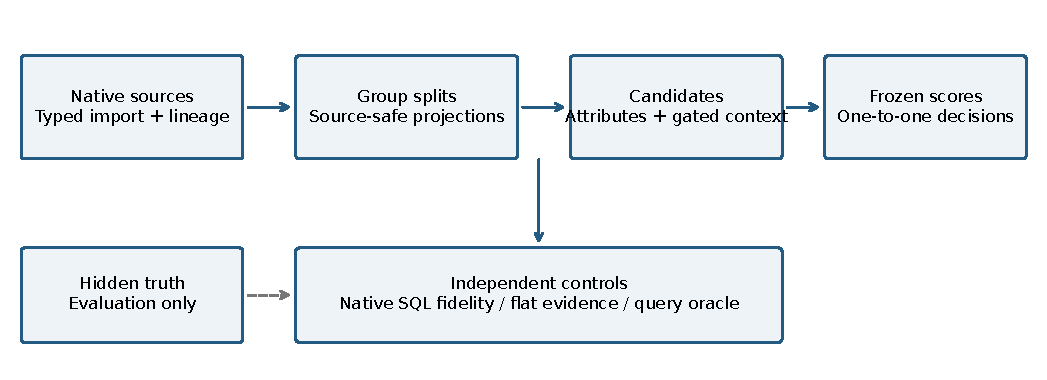
\includegraphics[width=\linewidth]{figures/architecture.pdf}
\caption{Implemented stages and independent controls. Evaluator truth is confined to splits, labels, reference checks and query oracles. Canonical links are created after scoring.}\label{fig:architecture}\end{figure}
Native extraction first retains source observations and valid relation endpoints. Mapping adds typed nodes and relation labels rather than replacing records with canonical entities. The larger expanded source graphs are SQLite-backed typed property graphs. The original WWI and the matching projections use NetworkX. This mixture supports local evaluation on the available machine; it is not a distributed database benchmark.

Every graph import checks node/edge counts, dangling endpoints, lineage presence and repeated-import idempotence. Independent native SQL joins define expected foreign-key relationship sets. Derived postal-prefix nodes in Olist are declared explicitly so that repeated geolocation observations are not mistaken for a single unique coordinate. DataCo master normalization uses the first source occurrence but retains every row observation and records disagreements. BPI event ordering preserves original trace ordinal, including timestamp ties or inversions, instead of silently rewriting the event history.

The matching layer creates separate namespaces for the source views and retains their own transaction histories. Generic adapters expose a Master--Transaction--Category projection. WWI also retains native master relations and independently inferred master anchors. The flat SQL context extractor joins the same permitted matching projection independently of graph traversal and is checked at feature and score levels. This flat control is distinct from the native-source SQL checks used by E1.

Lineage quality is $q(r)=\frac{1}{3}\sum_{f\in\{\mathrm{source\_table,batch,mapper}\}}\mathbb{1}[f(r)\text{ present}]$. It measures metadata completeness, not the probability that a row is correct. Weighted summaries use the smaller completeness value of the master and local transaction. WWI anchor contributions additionally use completeness of visible anchor attributes. Thus complete metadata can coexist with a misleading edge, and the robustness evaluation explicitly tests that case.

Decisions are sorted by descending score and apply frozen acceptance thresholds, same-type constraints and one-to-one endpoint use. Accepted records refer to generated canonical entities through an added view. Rejected, abstained and conflicting candidates remain in the decision audit. This design avoids source destruction but supports only the evaluated two-source, one-to-one problem. It is not a general transitive clustering algorithm for arbitrary duplicates.

\section{Datasets, Acquisition and Matching Tasks}
\begin{table}[t]\centering\small\begin{tabular}{lrrrl}
\toprule
Dataset & Native nodes & Native edges & Groups & Train / val. / test \\
\midrule
WWI & 249,786 & 274,856 & 240 & 143 / 48 / 49 \\
Olist & 1,569,937 & 1,775,243 & 2,913 & 1747 / 583 / 583 \\
DataCo & 267,103 & 607,478 & 1,500 & 900 / 300 / 300 \\
BPI2019 & 1,926,659 & 7,138,894 & 1,378 & 826 / 276 / 276 \\
\bottomrule
\end{tabular}

\caption{Native graph size versus matching population. Groups are original matching entities; each supplies two source-view observations. Native ingestion and matching scopes differ.}\label{tab:profiles}\end{table}
\subsection{Wide World Importers}
WWI is Microsoft's fictional business database sample~\cite{wwi}. The in-scope full-source graph contains six core tables, 249,786 nodes and 274,856 edges. Matching uses the preserved inventory of 13 suppliers and 227 stock items. Purchasing and warehouse/finance views have controlled aliases and source remapping; all relevant purchase and supplier-transaction rows and the first 5,000 primary-key-sorted stock-movement rows are retained in those original views. E1 includes the complete in-scope movement table. The fixed held-out set has 49 entities, including only three suppliers. Seeds alter aliases while retaining the original entity split.

QuantityPerOuter is exposed to every learned attribute comparator through equality, ratio and missingness features. It also converts purchased stock-item outer quantities to stock units for contextual comparison. Signed stock movements remain signed stock units; supplier-level outer quantities are a separate unit class. Supplier finance does not acquire invented quantities. Separate supplier and stock-owner transaction projections prevent mixed ownership.

\subsection{Olist}
Olist is the official Kaggle version-2 Brazilian e-commerce dataset~\cite{olist}. All nine source CSVs are imported, with explicit postal-prefix grouping nodes. Natural repeated customer observations are linked by customer\_unique\_id only in evaluator truth. An eligible group must have two distinct account observations with item histories. All 2,913 eligible groups are used; account selection is deterministic when more than two observations exist. Customers have city, state and postal prefix, not customer names. Up to 40 native order items are hash-selected per view. Price comes from the item row; quantity is the observed item-row count, while dates/status and product-category/seller-state information use declared source joins. Values are source units with unspecified currency, not paid customer spend.

Olist required an adapter amendment. A minimal diagnostic with product-category tags alone gave no supported test candidates. Before fitting expanded Olist models, native seller-state paths were added after inspecting test context availability. The prior fixture and amendment are retained. This makes Olist exploratory and partly test-informed at the adapter level, despite subsequent model/policy freezing.

\subsection{DataCo}
The DataCo version-5 publisher record describes structured supply-chain observations, clickstream data and a variable description file~\cite{dataco}. This study uses only the structured CSV, containing 180,519 rows and 53 columns. Publisher downloads returned HTTP 403; acquisition therefore used a documented third-party mirror. File hashes, schema and row counts are recorded, but equivalence to publisher bytes is not established.

The identity task consists of controlled customer aliases and disjoint hash-partitioned order histories, grouped by source Customer Id in evaluator truth. Of 10,075 eligible customers, 1,500 are selected by stable source-key hashing before alias perturbation. The selected set contains 900 training, 300 validation and 300 test entities. Visible names, segment and location fields are available; email/password fields are excluded from graph and matching attributes. Baseline abbreviations, typographical edits and optional missingness are controlled defects. They do not turn the source into independently annotated naturally dirty identity data. History features use native order dates, item totals/quantities, category/department and delivery status.

\subsection{BPI Challenge 2019}
BPI contains purchase-order event traces~\cite{bpi}. The publisher-linked XES has 251,734 cases and 1,595,923 events; publisher MD5 is checked. Full ingestion tests eight structural relation sets including case-vendor, event-case and directly-follows links. Matching selects all 1,378 eligible vendors, each represented by independently partitioned purchase cases, with 826/276/276 training/validation/test groups.

Vendor names, anonymized vendor IDs, company identifiers and original keys are excluded from matching text. The fields named name/category/brand by the shared model interface are modal spend-area, document-type and spend-classification descriptors derived separately from each view's history. Consequently, BPI tests the addition of detailed summaries beyond a coarse history-derived baseline, not a strong literal supplier-name matcher. Quantity is unavailable. Case amount is the first-event anonymized cumulative net worth, not the sum of cumulative event values or actual invoice payments. Activities use actual case events.

\subsection{WDC Products}
WDC uses all three official pairwise archives and their 27 hardness/development-size/unseen-product configurations~\cite{wdc,wdcsite}. The used files contain 155,957 pair observations, 10,422 distinct offers and 1,600 labelled groups. These counts refer to the used pairwise files and differ from the publisher's whole-benchmark counts. Each official test configuration has 4,500 pairs, including 500 positives. No official pair is silently removed. Nine hardness/size training settings with three seeds produce 27 model bundles, reused across three unseen-product variants: 81 seed/configuration evaluations rather than 81 independently fitted bundles.

Eighteen configurations have train-test and/or validation-test offer overlap. Fully unseen configurations have no such offer overlap. We preserve official results, flag both intersections and separately evaluate the offer-disjoint subset. Sizes can reuse a test pool; configuration means are descriptive correlated summaries. The supplied offer benchmark has no ERP foreign-key or transaction graph, so transaction context and E3 ERP queries are not applicable.

\section{Matching Models and Development Protocol}
\subsection{Attributes and the embedding reference}
The common attribute comparator uses 20 features: normalized character and token-sort similarity, token Jaccard, training-only character TF-IDF cosine, category/brand agreement, description similarity, price ratio/currency agreement, selected missingness flags, numeric/alphanumeric token overlap, explicit size compatibility/conflict/missingness, name-length ratio and digit missingness. WWI adds three packaging features, yielding 23. TF-IDF vocabulary is fitted on training records only. Sparse cosine calculations are processed in chunks to avoid a giant dense pair matrix. The common learners use scikit-learn~\cite{sklearn}.

Price/currency features do not convert currencies. Two empty currency strings are treated as equal by the attribute implementation, so price compatibility is not restricted to verified known currencies. Contextual numerical comparisons use declared unit classes, with missing/incompatible units handled explicitly. This distinction matters for interpreting source-unit amounts.

The pinned MiniLM model revision is recorded in the supplement. CPU inference uses a quantized ONNX artifact, 256-token truncation, batch size 64, attention-mask mean pooling and L2 normalization. Text is formed from allowed name/brand/description fields and truncated to 2,000 characters before tokenization. Original IDs, truth, prices and canonical keys are excluded. A 384-dimensional record embedding supplies a single cosine per pair; the embedding-only learner sees that scalar, and the augmented learner sees attributes plus the scalar. The encoder is not fine-tuned on these tasks.

\subsection{Context summaries and gates}
Generic context has 16 dimensions: category/activity cosine, degree similarity, distinct shared tags, weighted support fraction, date-mean/span similarity, quantity-mean/deviation similarity, amount-mean/deviation similarity, date availability, quantity/amount unit compatibility, category contradiction and context availability. Moments are weighted by lineage completeness. Generic support requires at least two distinct projected category tags and weighted support of at least one. Tags prefixed for missing category values can count as support. Thus two tags need not be two known informative categories or two independently resolved entities.

WWI combines five native master-context dimensions, 15 transaction-summary dimensions and its original independent-anchor gate. Anchors are inferred by unique exact normalized names, compatible categories and entity types, with candidate endpoints excluded. Stock-to-supplier and co-supplied-stock relations provide typed native context. At least two distinct inferred master anchors and weighted support of one are required. QuantityPerOuter is excluded from anchor inference even though attribute baselines and contextual conversion can use it.

\subsection{Candidates and the ambiguous stratum}
WWI preserves the original token-prefix/category block, without a per-left K cap in the E2 common pool, subject to a two-million-pair guard. Other graph tasks use the bounded K=32 common pool. The attribute-defined ambiguous stratum includes a pair when normalized character similarity is below 0.95 or when its left record has more than one candidate with token-sort similarity at least 0.65. All compared methods use the same stratum. It is a candidate-conditioned diagnostic rather than a sample of every possible pair.

A separate bounded retrieval policy tests K=8,16,32 on validation, with target recall 0.95, at most 12 keys per record, posting cap 8K and two-million output guard. Deterministic hashing orders postings, then visible name similarity ranks the pool. The smallest K reaching the target is selected; otherwise the best validation recall is selected with a smaller-K tie break. WWI selects K=8; the other graph tasks use K=32 and fail to reach the target. WDC E2 instead evaluates official test pairs; its E5 offer-retrieval workload is separate.

\subsection{Training, calibration and policy separation}
Canonical groups are split before aliases. Generic splits are 60/20/20 with deterministic hashing; WWI's original splits are preserved. Within validation, groups are partitioned into selection, calibration and policy roles. A pair is eligible for a role only when both endpoints belong to that role; cross-role pairs are omitted. Selection compares the same five estimators for each learned family: standardized class-balanced logistic regression with C=0.1,1,10 and class-balanced 160-tree random forests with depth 8 or 16 and minimum leaf size two. Selection uses its own best weighted F1 threshold and catalog-order tie break. Logistic iteration limit is 1,500; random forests use two jobs.

Role class weights restore the full-validation candidate prevalence, using $\pi/\pi_r$ for positives and $(1-\pi)/(1-\pi_r)$ for negatives. This is validation-only reweighting, not correction to a known test prior. The chosen trained estimator is calibrated on a separate role by logistic regression on clipped probability logits, with C=$10^6$ and iteration limit 1,000. A final acceptance threshold maximizes weighted F1 on the policy role, preferring the higher threshold on ties. Rejection is bounded by 0.10 and the acceptance threshold. Estimators, calibrators, policies, code/input hashes and timestamps are persisted before test-label scoring. Small disjoint roles can still yield unstable selection and calibration.

\subsection{Comparators and ablations}
Exact matching requires normalized-name equality, category agreement and nonmissing name; fuzzy matching uses token-sort similarity. Attributes, embedding-only and augmented attributes are learned references. B5 uses gated graph context and B4 independently extracts identical evidence through SQL, using the same context estimator and policy. NoContext shares the attribute model and threshold. NoGate evaluates the weighted learner without attribute fallback, using its own policy threshold; it is not a separately trained gate-free learner.

NoSupport trains without explicit support features while retaining the original gate at final scoring. OneHop uses local transaction activity/numerical evidence without category traversal in generic adapters; its meaning concerns the normalized projection rather than native process depth. WWI applies its typed native one-hop transformation as well. NoTransactions removes the entire 15-dimensional transaction block in WWI, but only date/numerical/unit dimensions in generic adapters, leaving category/activity/degree context. It therefore has adapter-specific semantics. UnitWeights supplies unit-weight features to the frozen weighted estimator and policy; it is an input-weight stress test, not a retrained provenance ablation. A separately retrained WWI comparison exists in the preserved earlier study, not in this contrast.

\section{Experimental Design and Measurement}
E1 compares complete in-scope native imports with independent relational reference sets. E2 evaluates 12 graph seed runs with 13 methods and 81 WDC seed/configuration cells with five methods. We report candidate-conditioned ambiguous F1, all-candidate end-to-end F1, subgroup/retained-positive counts and final accepted-link audits. There is no pooled cross-dataset performance number because these tasks expose different attributes, truth constructions and graph semantics.

For each graph seed, a paired bootstrap resamples canonical groups present in the ambiguous candidate set 1,000 times. If sampled multiplicities are $m_g$, a same-group pair has weight $m_g$; a pair connecting distinct groups $g,h$ has weight $m_gm_h$. The same weights are applied to both compared classifiers. Percentiles 2.5 and 97.5 are descriptive intervals for the paired F1 difference. This endpoint-multiplicity procedure is specified explicitly rather than presented as independent pair resampling. Three alias seeds share source entities, and their intervals are not pooled into a confirmatory confidence interval. No multiplicity-adjusted hypothesis testing or preregistered significance claim is made.

E3 executes eight dataset-adapted templates under unreconciled, predicted and oracle identity maps. Independently implemented SQL and graph answers must agree exactly under each map. Oracle truth is used only for evaluation. Source UIDs normalize answer tuples, and monetary sums use cent-rounded source units. Q2/Q4 are source-local controls; Q1/Q3/Q5/Q6/Q7/Q8 depend on reconciliation. The adapted templates are not 32 independent business workloads. WWI separately retains eight native queries with its original purchasing, stock, finance and provenance semantics.

E4 reuses frozen clean candidate pairs, models and policies under 12 graph conditions: clean, no anchors/support, additional attribute noise 30/50\%, optional missingness 10/30/50\%, edge removal 15/30\%, typed misleading rewiring 15/30\%, and lineage missingness 30\%. WDC has six attribute-only conditions. Typed rewiring stays within entity kind, silo and split; logs remain evaluator-only. These stress rates are controlled scenarios, not measured production defect prevalence. Frozen-pair tests isolate score sensitivity but do not test blocking under corruption. Calibration uses all candidate pairs, raw/calibrated Brier score, log loss and ten equal-width-bin expected calibration error (ECE). Coverage and selective risk count accepted and rejected pairs before one-to-one constraints.

E5 uses three targets, 1,000/10,000/100,000 projected graph nodes or WDC offers, with three trials each: 45 main trials. Complete graph units may slightly exceed targets. Growth initially adds independent test groups; later growth creates replicas. True-pair denominators include cross-replica pairs belonging to the same original entity, with no copy-suffix feature. Graph queries use a common per-copy oracle identity map, independently of predicted matching quality. One warmup and five measured executions produce each trial's p50/p95; graph preparation and SQL loading/indexing are timed separately. Process RSS is sampled every 50 ms, with absolute peak and increment. Supplemental scorer-only and canonicalization timings do not replace the main end-to-end trials.

\section{Results}
\subsection{E1: source fidelity}
All four native graph imports match their expected in-scope source relationships, have no dangling edges, retain full lineage metadata and pass repeated-edge-import idempotence checks. Table~\ref{tab:profiles} reports sizes. Olist tests ten native/derived relations, DataCo six, BPI eight, and WWI eight independent foreign-key controls. WDC verifies unique offer identities, pair schema/counts, evaluator-label exclusion and official split-member checksums rather than ERP graph relations. Exactness is relative to the implemented source mappings and SQL reference definitions, not proof that publishers' data are correct or that all conceivable business semantics were represented.

\subsection{E2: contextual matching and representation parity}
\begin{table}[t]\centering\small\begin{tabular}{lrrrr}
\toprule
Method & WWI & Olist & DataCo & BPI \\
\midrule
Exact & 0.3402 & 0.7502 & 0.1994 & 0.0538 \\
Fuzzy & 0.7145 & 0.1039 & 0.2001 & 0.0639 \\
Attributes & 0.7688 & 0.6919 & 0.6962 & 0.1242 \\
Embedding & 0.4157 & 0.2327 & 0.2594 & 0.0840 \\
Attributes + embedding & 0.7626 & 0.7414 & 0.6962 & 0.1492 \\
Flat SQL context & 0.7888 & 0.7842 & 0.6750 & 0.5734 \\
Gated graph context & 0.7888 & 0.7842 & 0.6750 & 0.5734 \\
No context & 0.7688 & 0.6919 & 0.6962 & 0.1242 \\
No gate & 0.7763 & 0.7806 & 0.6710 & 0.5734 \\
No support features & 0.7879 & 0.7913 & 0.6780 & 0.5465 \\
No transaction summaries & 0.7887 & 0.7474 & 0.6790 & 0.4264 \\
One hop & 0.7688 & 0.6919 & 0.6946 & 0.4827 \\
Unit-weight inputs & 0.7440 & 0.7842 & 0.6750 & 0.5734 \\
\bottomrule
\end{tabular}

\caption{Mean F1 over three seeds on common attribute-defined ambiguous candidates. These are conditional pair results; generic and WWI ablations have the distinctions specified in Section 6.}\label{tab:match}\end{table}
Table~\ref{tab:match} shows that context changes mean ambiguous F1 from \FWwiAttr{} to \FWwiGraph{} on WWI, \FOlistAttr{} to \FOlistGraph{} on Olist, \FDataCoAttr{} to \FDataCoGraph{} on DataCo, and \FBpiAttr{} to \FBpiGraph{} on BPI. The respective differences are +0.0200, +0.0923, -0.0212 and +0.4492. DataCo contradicts universal contextual improvement. On Olist, exact matching reaches 0.7502, exceeding learned attributes at 0.6919; the learned attribute reference is therefore not the strongest control on every dataset.

\begin{figure}[t]\centering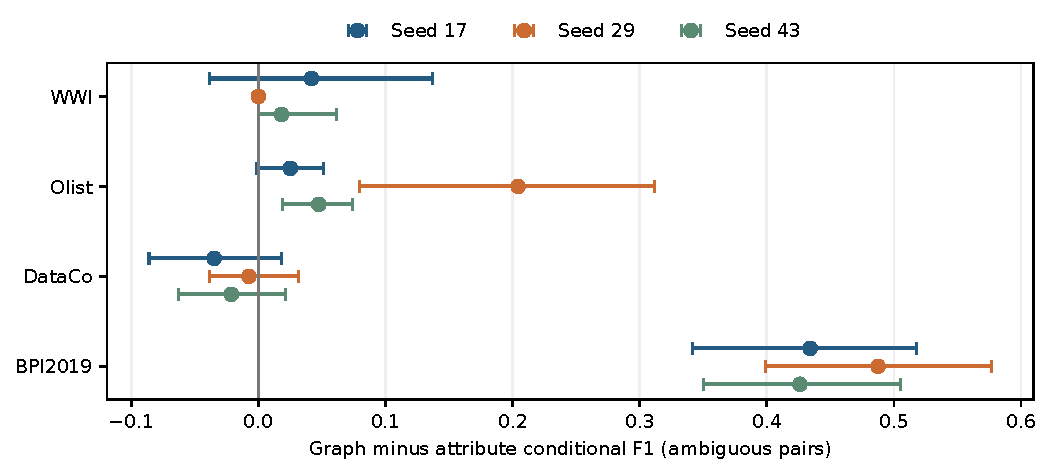
\includegraphics[width=\linewidth]{figures/context_effects.pdf}
\caption{Per-seed graph-minus-attribute effects and paired group-resampling percentile intervals. Seeds share original source populations. BPI effects are conditional on its coarse descriptor baseline.}\label{fig:effects}\end{figure}
\begin{table}[t]\centering\small\begin{tabular}{lrrrr}
\toprule
Dataset & Seed & $\Delta$ F1 & 2.5\% & 97.5\% \\
\midrule
WWI & 17 & +0.0419 & -0.0386 & +0.1371 \\
WWI & 29 & +0.0000 & +0.0000 & +0.0000 \\
WWI & 43 & +0.0183 & +0.0000 & +0.0612 \\
Olist & 17 & +0.0252 & -0.0015 & +0.0511 \\
Olist & 29 & +0.2043 & +0.0795 & +0.3119 \\
Olist & 43 & +0.0476 & +0.0190 & +0.0739 \\
DataCo & 17 & -0.0347 & -0.0860 & +0.0182 \\
DataCo & 29 & -0.0074 & -0.0388 & +0.0315 \\
DataCo & 43 & -0.0212 & -0.0631 & +0.0213 \\
BPI2019 & 17 & +0.4341 & +0.3416 & +0.5177 \\
BPI2019 & 29 & +0.4876 & +0.3993 & +0.5764 \\
BPI2019 & 43 & +0.4261 & +0.3500 & +0.5049 \\
\bottomrule
\end{tabular}

\caption{Exact per-seed ambiguous F1 effects with paired bootstrap percentile endpoints. No pooled or multiplicity-adjusted confidence statement is made.}\label{tab:ci}\end{table}
WWI has one seed with identical graph and attribute decisions and two with small gains; its intervals are broad relative to the mean effect. Olist's gains vary strongly across aliases, with the seed-17 interval crossing zero. All three DataCo point estimates are negative and their intervals cross zero. BPI's three effects are positive with intervals above zero, but the task compares detailed history to weak coarse history descriptors and cannot establish analogous gains for real supplier-name matching. Figure~\ref{fig:effects} and Table~\ref{tab:ci} make this heterogeneity visible.

Flat and graph context features and scores agree within $10^{-12}$. Accordingly, B4 and B5 F1 are identical. This supports the inference that the contextual evidence can be reproduced relationally. It refutes an interpretation in which this experiment demonstrates a graph storage format itself improving classification. Generic clean lineage weights are all one, so identical UnitWeights results on those datasets do not establish the usefulness of provenance weighting. WWI's differing anchor-attribute completeness explains its nonidentical unit-weight contrast.

\begin{table}[t]\centering\small\begin{tabular}{lrrrrr}
\toprule
Dataset & Groups & Candidates & Block R & Attr. F1 & Graph F1 \\
\midrule
WWI & 49 & 1314--1411 & 1.000 & 0.797 & 0.826 \\
Olist & 583 & 8815--8816 & 0.821 & 0.654 & 0.725 \\
DataCo & 300 & 8857--9016 & 0.874 & 0.674 & 0.649 \\
BPI2019 & 276 & 7850--8049 & 0.755 & 0.110 & 0.490 \\
\bottomrule
\end{tabular}

\caption{Full-positive-universe pair F1, before one-to-one constraints. Candidate ranges are over seeds; Block R is mean candidate recall. Attr./Graph columns are end-to-end F1, not the ambiguous F1 in Table~\ref{tab:match}.}\label{tab:pipeline}\end{table}
Blocking retains all WWI positives in the preserved E2 pool, but only mean recalls of 0.821, 0.874 and 0.755 on Olist, DataCo and BPI. End-to-end graph F1 is 0.826, 0.725, 0.649 and 0.490, respectively. These values expose retrieval losses hidden by candidate-conditioned reporting. Context improves the full-pipeline pair score on WWI/Olist/BPI and reduces it on DataCo within this evaluated setup. One-to-one decisions subsequently change which links survive.

\begin{table}[t]\centering\small\begin{tabular}{lrrr}
\toprule
Dataset & Accepted & True links & False merges \\
\midrule
WWI & 107 & 106 & 1 \\
Olist & 1092 & 1055 & 37 \\
DataCo & 636 & 574 & 62 \\
BPI2019 & 372 & 318 & 54 \\
\bottomrule
\end{tabular}

\caption{Clean graph-method links accepted after one-to-one constraints, summed across seed trials. Repeated seeds reuse source populations; counts are trial outcomes, not independent production events.}\label{tab:identity}\end{table}
The final decision audit finds 1 false merge among 107 accepted WWI links, 37 among 1,092 Olist links, 62 among 636 DataCo links, and 54 among 372 BPI links. Stronger conditional F1 does not eliminate erroneous canonical links. These postconstraint counts must not be interchanged with preconstraint false-positive counts from perturbation tables. The system retains evidence and decisions to make such errors inspectable; it does not automatically guarantee harmless downstream effects.

\subsection{WDC: official configurations and clean generalization}
\begin{table}[t]\centering\small\begin{tabular}{lr}
\toprule
Method & Mean F1 \\
\midrule
Exact & 0.0000 \\
Fuzzy & 0.3477 \\
Attributes & 0.5369 \\
Embedding & 0.3919 \\
Attributes + embedding & 0.5584 \\
\bottomrule
\end{tabular}

\caption{Descriptive mean F1 over nine fully unseen configurations and three training seeds. Development sizes reuse test pools; the 27 observations per method are not independent samples.}\label{tab:wdcmean}\end{table}
On fully unseen cells, attribute F1 is \WdcAttr{}, embedding-only F1 is \WdcEmb{} and augmented F1 is \WdcAug{}. The augmented-minus-attribute difference is 0.0215. A cosine feature can complement lexical features here, while the cosine-only model is weaker. We do not attach a pooled confidence interval to correlated configuration means or select an unseen variant by test performance.

Table~\ref{tab:wdcall} in Appendix A reports all 27 official cells with both overlap counts. Small 0\%-unseen configurations illustrate why checking only training overlap is insufficient: training-test intersection can be zero while validation-test intersection is nonzero. The offer-disjoint subset is saved with exact pair/positive denominators and its own metrics. It is an audited diagnostic subset rather than a replacement official benchmark or a newly sampled test distribution.

\subsection{E3: query correctness and the limits of parity}
\begin{table}[t]\centering\small\begin{tabular}{lrrrr}
\toprule
Query & WWI & Olist & DataCo & BPI \\
\midrule
Q1 & 0.800 & 0.794 & 0.739 & 0.561 \\
Q2 & 1.000 & 1.000 & 1.000 & 1.000 \\
Q3 & 0.845 & 0.743 & 0.747 & 0.528 \\
Q4 & 1.000 & 1.000 & 1.000 & 1.000 \\
Q5 & 0.998 & 0.729 & 0.742 & 0.603 \\
Q6 & 0.832 & 0.743 & 0.747 & 0.528 \\
Q7 & 0.816 & 0.741 & 0.745 & 0.560 \\
Q8 & 0.931 & 0.729 & 0.742 & 0.594 \\
\bottomrule
\end{tabular}

\caption{Three-seed mean answer-set F1 for predicted identities on eight adapted templates. SQL and graph answers are exactly equal under unreconciled, predicted and oracle identities; oracle accuracy is one. Q2/Q4 are source-local controls.}\label{tab:queries}\end{table}
All 288 adapted query rows pass SQL/graph exactness, and all oracle workloads are nonempty. Source-local Q2/Q4 attain F1=1 irrespective of reconciliation. Identity-sensitive tasks recover answers absent under the unreconciled view, but predicted maps leave substantial errors. For example, Olist Q6 identity-pair F1 is 0.743 and BPI Q6 is 0.528. BPI Q5 transaction-link F1 is 0.603, illustrating that query accuracy weights the consequences of errors differently from pair F1. No single average is used to collapse these distinct workloads.

Q1 links matched entities sharing observed projected categories; Q3 attributes B-side amount/count to A; Q5 links positive-value B transactions; Q6 returns identities; Q7 groups B-side amount/count by visible tags; Q8 returns source-table lineage for reconciled transactions. Q7's category vocabularies can overlap, so summing across tag classes double-counts observations and is not a global spend rollup. BPI amounts remain anonymized case values and DataCo/Olist amounts have unspecified currency. The additional 72 native WWI query rows retain its purchasing, movement and finance semantics, including Q7 category totals and Q8 finance-path lineage.

SQL/graph equality establishes consistent execution of the chosen identities and mappings. The oracle comparison establishes accuracy relative to evaluator truth. Neither implies that a wrong identity map is correct simply because two implementations return the same result. This separation is central to interpreting integrated systems.

\subsection{E4: defects, ablations and calibration}
\begin{figure}[t]\centering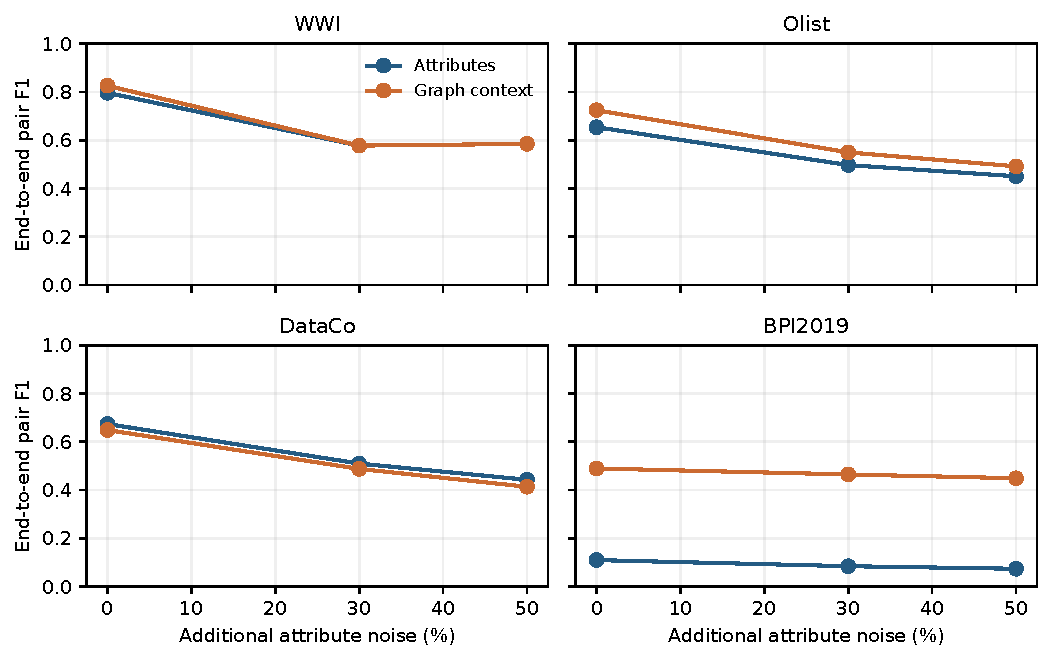
\includegraphics[width=\linewidth]{figures/attribute_stress.pdf}
\caption{Additional attribute-noise stress on frozen candidates. End-to-end pair F1 includes clean retrieval omissions; retrieval itself is not rerun under defects. Curves are three-seed means, not production failure forecasts.}\label{fig:stress}\end{figure}
The graph runs yield 1,872 method/scenario rows, and WDC yields 2,430. Figure~\ref{fig:stress} shows the clean/attribute-noise contrast; the supplement reports all conditions. Context can preserve matching evidence when attributes deteriorate, but benefits depend on available histories, support definitions and the learned policy. Edge removal changes summary completeness; misleading rewiring can leave abundant metadata while attaching incorrect observations. A completeness-based weight cannot detect every such defect.

Clean ablations already qualify the mechanism. Removing numerical/date/unit transaction summaries reduces BPI ambiguous mean F1 from 0.5734 to 0.4264; generic activity/category evidence remains. WWI's transaction ablation removes its entire transaction block and changes little, from 0.7888 to 0.7887, so these clean WWI gains cannot be attributed to that block alone. Removing the gate changes WWI from 0.7888 to 0.7763, while clean BPI is unchanged. NoSupport can slightly exceed the full model on Olist and DataCo. These results reject a simple claim that every component consistently helps every adapter.

\begin{table}[t]\centering\small\begin{tabular}{lllrrr}
\toprule
Dataset & Method & Mode & Brier & Log loss & ECE \\
\midrule
BPI2019 & Attr. & calibrated & 0.0251 & 0.1120 & 0.0021 \\
BPI2019 & Attr. & raw & 0.1711 & 0.4903 & 0.3301 \\
BPI2019 & Graph & calibrated & 0.0149 & 0.0541 & 0.0052 \\
BPI2019 & Graph & raw & 0.0180 & 0.0725 & 0.0190 \\
DataCo & Attr. & calibrated & 0.0129 & 0.0407 & 0.0088 \\
DataCo & Attr. & raw & 0.0213 & 0.0777 & 0.0366 \\
DataCo & Graph & calibrated & 0.0138 & 0.0443 & 0.0073 \\
DataCo & Graph & raw & 0.0189 & 0.0678 & 0.0291 \\
Olist & Attr. & calibrated & 0.0211 & 0.0850 & 0.0111 \\
Olist & Attr. & raw & 0.0765 & 0.2297 & 0.1332 \\
Olist & Graph & calibrated & 0.0189 & 0.0779 & 0.0182 \\
Olist & Graph & raw & 0.0791 & 0.2372 & 0.1403 \\
WWI & Attr. & calibrated & 0.0077 & 0.0272 & 0.0078 \\
WWI & Attr. & raw & 0.0098 & 0.0418 & 0.0104 \\
WWI & Graph & calibrated & 0.0082 & 0.0300 & 0.0079 \\
WWI & Graph & raw & 0.0094 & 0.0420 & 0.0102 \\
\bottomrule
\end{tabular}

\caption{All-candidate calibration diagnostics, averaged over seeds. Lower values are better. Discrimination, calibrated losses, ECE and postconstraint link correctness are distinct assessments.}\label{tab:calibration}\end{table}
Sigmoid calibration lowers mean raw Brier/log-loss/ECE for the reported attribute and graph methods on these candidate sets. Comparing calibrated methods still gives mixed results: DataCo's attribute Brier is lower than graph Brier, and WWI's calibrated graph losses do not dominate attributes. Olist graph ECE is higher than attribute ECE despite lower graph Brier/log loss. These are descriptive finite-sample diagnostics under different prevalences. They do not establish calibration on an unseen deployment population or error guarantees for an acceptance threshold. The supplement includes coverage/risk sources so acceptance, rejection and abstention can be inspected together.

\subsection{E5: computational scale and retained positives}
\begin{table}[t]\centering\small\setlength{\tabcolsep}{4pt}\begin{tabular}{lrrrrrrr}
\toprule
Dataset & Target & Actual & Match rec. & Pairs & Block R & Seconds & RSS GiB \\
\midrule
WWI & 1k & 1,021 & 36 & 132 & 1.000 & 0.25 & 0.32 \\
WWI & 10k & 10,722 & 96 & 356 & 1.000 & 1.87 & 0.37 \\
WWI & 100k & 100,729 & 974 & 3,896 & 0.705 & 24.46 & 0.70 \\
Olist & 1k & 1,000 & 414 & 2,309 & 0.966 & 0.57 & 0.32 \\
Olist & 10k & 10,001 & 4,308 & 47,913 & 0.722 & 7.56 & 0.48 \\
Olist & 100k & 100,001 & 43,176 & 687,264 & 0.397 & 109.13 & 2.91 \\
DataCo & 1k & 1,011 & 112 & 1,312 & 0.946 & 0.71 & 0.66 \\
DataCo & 10k & 10,001 & 1,150 & 17,074 & 0.820 & 6.58 & 0.70 \\
DataCo & 100k & 100,012 & 11,470 & 179,974 & 0.594 & 69.57 & 1.49 \\
BPI2019 & 1k & 1,032 & 50 & 270 & 0.920 & 0.50 & 1.08 \\
BPI2019 & 10k & 10,023 & 560 & 8,231 & 0.767 & 4.50 & 1.11 \\
BPI2019 & 100k & 100,014 & 5,566 & 88,716 & 0.172 & 47.62 & 1.49 \\
WDC & 1k & 1,000 & 1,000 & 12,638 & 0.990 & 0.96 & 2.00 \\
WDC & 10k & 10,000 & 10,000 & 160,137 & 0.837 & 18.74 & 2.11 \\
WDC & 100k & 100,000 & 100,000 & 1,606,844 & 0.336 & 373.05 & 3.27 \\
\bottomrule
\end{tabular}

\caption{All 15 dataset/target points: medians over three main trials. Graph Actual counts projected nodes; WDC Actual counts offers. Match rec. is the number of matching observations. Seconds cover the implemented main pipeline; peak RSS is absolute process memory.}\label{tab:scale}\end{table}
All 45 trials complete under the declared graph memory budget. At the largest target, main median wall time is 24.46 s for WWI, 109.13 s for Olist, 69.57 s for DataCo, 47.62 s for BPI and 373.05 s for WDC. Absolute median peak RSS reaches 3.27 GiB on WDC. These timings refer to local projected workloads, not to full native graph sizes or production ingestion of 100,000 new independent masters.

\begin{figure}[t]\centering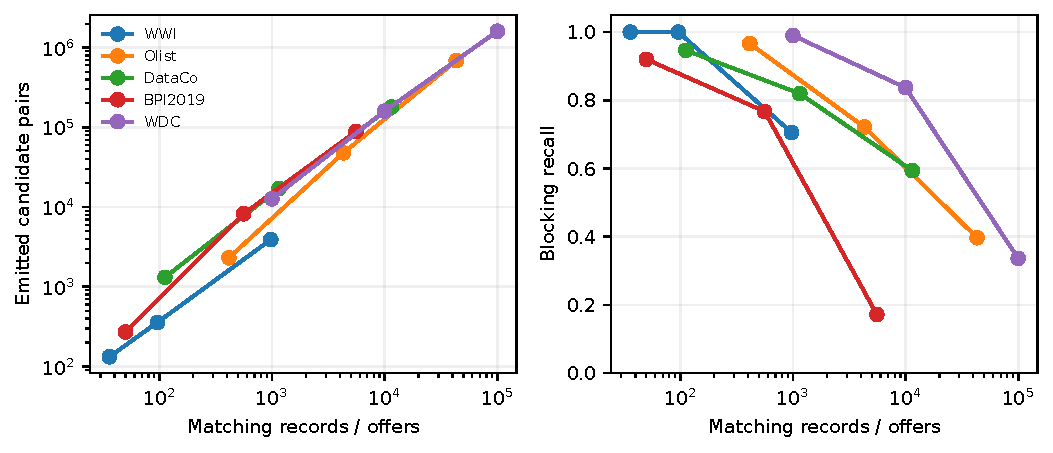
\includegraphics[width=\linewidth]{figures/blocking.pdf}
\caption{Emitted candidates and blocking recall plotted against matching records, avoiding confusion between graph nodes and matchable entities. Bounded output can grow modestly while recall deteriorates.}\label{fig:blocking}\end{figure}
At the largest target, blocking recall is 0.705 for WWI, 0.397 for Olist, 0.594 for DataCo, 0.172 for BPI and 0.336 for WDC. Cross-replica positives increase the complete true-pair universe, while bounded posting retrieval and emitted-pair caps omit many of them. Figure~\ref{fig:blocking} therefore supports a trade-off between work and retained positives, not a successful recall-preserving scale claim. Observed candidate-count slopes describe capped output at three points; internal ranking/pool work is not proven subquadratic.

\begin{table}[t]\centering\small\begin{tabular}{llrr}
\toprule
Dataset & Engine & p50 ms & p95 ms \\
\midrule
BPI2019 & graph & 349.45 & 375.80 \\
BPI2019 & sql & 1378.93 & 1393.95 \\
DataCo & graph & 415.09 & 476.25 \\
DataCo & sql & 1668.25 & 1826.90 \\
Olist & graph & 238.08 & 289.30 \\
Olist & sql & 1296.64 & 1341.63 \\
WWI & graph & 193.26 & 224.31 \\
WWI & sql & 768.46 & 841.87 \\
\bottomrule
\end{tabular}

\caption{Largest-target warmed query batches. Values are medians of per-trial p50/p95 over five measured executions; graph adjacency and SQL loading/index preparation are separately measured. Both engines use the same per-copy oracle identity map.}\label{tab:latency}\end{table}
The prepared graph implementation executes the eight-template batch faster than the indexed SQLite control at these largest projected points (Table~\ref{tab:latency}). This is an implementation-specific observation with common oracle identities. It does not compare commercial graph and relational optimizers, cold end-to-end costs, independent production workload mixes or distributed systems. Preparation costs, individual-template latencies and all trials remain available for different workload interpretations.

Supplemental scorer timing compares attributes, flat context and graph context on identical feature matrices after one warmup and three repetitions. Graph targets count projected nodes; WDC supplemental targets count 1,000/10,000/100,000 input pair rows obtained by tiling an official frozen feature matrix. Those WDC targets do not count 100,000 source offers. Greedy canonicalization costs are measured separately. These isolated costs identify components but cannot be used as an end-to-end context-overhead ratio because feature construction is excluded.

\section{Discussion and Implications}
\subsection{Answers to the planned hypotheses}
RQ1/H1 is \textbf{supported within the declared mappings}: native reference sets and lineage are exact, exceeding the planned 99\% relationship target. RQ2/H2 is \textbf{uncertain as a robust primary claim}: WWI mean ambiguous uplift is about 0.02, but seed effects and intervals do not establish a stable positive population effect. The expanded evidence is mixed, including negative DataCo. RQ3/H3a is \textbf{supported for evaluated alias-affected tasks}, with remaining errors; H3b is \textbf{supported as execution parity under the same map}, without certifying wrong identities. RQ4/H4 is \textbf{mixed and adapter-dependent}: degradation and gate/ablation behavior vary, and completeness is not correctness. RQ5/H5 is \textbf{partially supported for measured feasibility and capped output}, but positive recall deteriorates, isolated scorer costs are not end-to-end overhead, and subquadratic computation is not established. These statuses describe executed exploratory evidence, not confirmatory acceptance of the original prospective hypotheses.
\subsection{What the evidence supports}
Typed source integration and auditable identity decisions are achieved for the declared mappings. Context contributes useful information in several evaluated tasks, particularly where the attribute interface is coarse, but its benefit is conditional. The negative DataCo result and the variable Olist seed effects matter as much as the positive BPI contrast. A practical deployment should test attributes, context and retrieval on its own identity task rather than infer a universal gain from these datasets.

Graph and relational context parity supplies an unusually direct diagnostic. If feature equality fails, a matching difference may reflect divergent extraction rather than modeling. If features and scores agree, a predictive difference cannot be credited to storage representation. The graph remains useful as a typed evidence organization, but that usefulness has not been established through a human study or operational adoption metric here.

The query experiments expose another separation: representation correctness is not identity correctness. A query engine can faithfully execute a false canonical map. Conversely, a correct identity pair can have a disproportionate effect on a large transaction history. Recording source-level answers and their denominators makes these consequences visible. It also prevents aggregate amount differences from being described as actual financial loss when currencies, payments or causal business outcomes were not measured.

\subsection{Where the present method is weak}
The generic support gate counts projected tag overlap, including explicit missingness markers. It can therefore overstate available informative context. An informative-tag gate, trained support estimator or independently inferred anchors would be reasonable future changes, but they have not been evaluated in this completed run. Provenance completeness likewise cannot stand in for source correctness. A future system would need empirically grounded source-quality signals and evaluations of misleading yet complete evidence.

The embedding reference is deliberately accessible but narrow. A single cosine cannot exploit every interaction available to a fine-tuned pair model. Its positive WDC increment motivates richer attribute references without claiming the present context method surpasses them. Related neural methods require separate implementation, compatible split controls and equal tuning resources before a comparative claim is justified.

Retrieval is the clearest scale limitation. Completion time and memory remain feasible at the measured points, but positive recall collapses for several replicated workloads. Improving candidate recall under growing duplicate multiplicity is a distinct research problem. A graph scorer that never sees those omitted positives cannot solve it. Reporting both matching records and graph nodes makes that failure interpretable.

\section{Threats to Validity}
\textbf{Construct validity.} The five datasets do not instantiate the same identity problem. WWI aliases are simulated, Olist repeats are natural account observations, DataCo/BPI use controlled views, and WDC is an offer-pair benchmark. BPI attributes are coarse history summaries. Source-unit aggregates, category tags and adapter-specific ablations must be interpreted according to those constructions. Oracle truth expresses original source identity, not independently adjudicated dirty-record identity on every source.

\textbf{Internal validity.} Group-before-alias splits, evaluator-only truth, train-only vocabulary and disjoint validation roles reduce direct leakage. They do not erase test-informed Olist adapter development, small validation roles, shared source populations across seeds, candidate conditioning or role prevalence shift. Eighteen WDC cells have observed offer overlap. Official results with overlap are descriptive; fully unseen and offer-disjoint diagnostics provide cleaner evidence within their stated denominators.

\textbf{Statistical validity.} There are only three alias/training seeds. WWI has 49 held-out groups and only three suppliers. Correlated pair data are addressed with an explicitly specified paired endpoint-multiplicity bootstrap, but intervals are exploratory and no familywise testing is claimed. Test pools repeat across WDC configurations. Seed means and trial medians are not independent population estimates. Timing percentiles from five warm repetitions are coarse measurements and cannot characterize tail latency at deployment scale.

\textbf{External validity.} Public datasets, controlled aliases, capped histories, one-to-one identity and replication-based scale do not represent every ERP workload. No human study, expert trust assessment, production deployment or organizational benefit evaluation was performed. DataCo mirror acquisition limits publisher-byte provenance. CPU-only local measurements do not generalize to different database engines, hardware, concurrency or distributed deployments.

\textbf{Implementation validity.} Independent metric recomputation, frozen replay and SQL/graph controls detect many errors but can share abstractions or source mapping assumptions. The original primary run has a separate fresh-environment retraining replication. The expanded study has verified frozen-model replay, not an independent fresh retraining replication. This distinction remains explicit in the paper and archive.

\section{Reproducibility, Amendments and Responsible Release}
The expanded run records configuration, source/code hashes, model choices, thresholds, all seed/configuration predictions, query denominators, perturbations and timing trials. Independent verification reports 3,136 passing checks and 36 passing control tests. Recomputed metrics agree with saved values, all 12 graph seed runs and 81 WDC seed/configuration cells replay frozen scores, and query controls execute afresh. The manuscript generator reads those artifacts without fitting models or changing experimental measurements. A quantitative claim registry links each generated table, figure and headline value to source hashes and aggregation rules.

The interrupted WWI run was resumed while preserving fitted models. SQL Q1 was optimized by deduplicating master/tag incidence before the identity join; all WWI E5 trials were rerun, and earlier six timings/code were retained. Olist's seller-state support amendment precedes its first expanded training but follows a test-context diagnostic. A later Olist lineage repair changed the projected transaction origin to the order-item table, reran query controls and all nine E5 trials, preserved frozen models and verified score replay. Prior measurements and amendment hashes remain archived. These corrections improve implementation fidelity while precluding a preregistered narrative.

No participants were recruited and no human study was performed. DataCo credentials/contact fields are excluded from graph/model attributes; raw source reference storage remains local. Acquisition manifests identify source versions, mirror limitations and publisher-linked BPI checks. Dataset and model licenses differ: Olist carries CC BY-NC-SA 4.0, DataCo and BPI publisher metadata indicate CC BY 4.0, and the MiniLM model card indicates Apache 2.0. Raw datasets, source databases, evaluator truth and downloaded model weights are excluded from the private manuscript source package. Public redistribution, code licensing and an archival DOI are not claimed to be complete.

\section{Conclusion}
The evaluated prototype connects typed source ingestion, attribute/context matching, constrained canonical views and independent query controls across five datasets. Exact source/reference checks and flat SQL/graph parity establish implementation properties within the declared mappings. Context improves some evaluated identity tasks but harms DataCo on average; BPI's large gain depends on a coarse history-derived baseline. Query consequences remain task-specific, accepted false merges persist, and bounded retrieval loses many positives at larger replicated workloads. These findings support traceable, qualified contextual reconciliation and a reproducible evaluation framework. Future evidence should test stronger learned references, informative support, recall-preserving retrieval, independent full-study retraining and real operational use before broader claims are made.

\section*{Acknowledgment and AI Assistance}
OpenAI Codex (GPT-6) assisted with software implementation, experiment orchestration, result checking, manuscript drafting across all sections, bibliography organization, and generation of tables, scientific plots and publication files. Reported numerical results derive from executed local scripts and saved artifacts. This disclosure describes the assistance used; human author approval, authorship details, funding and competing-interest declarations remain to be supplied before submission.

\clearpage
\appendix
\section{All Official WDC Pairwise Configurations}
\begin{table}[htbp]\centering\footnotesize\setlength{\tabcolsep}{4pt}\begin{tabular}{rlrrrrrr}
\toprule
Hard & Size & Unseen & Attr. & Emb. & Attr.+emb. & Train $\cap$ test & Val. $\cap$ test \\
\midrule
20 & small & 0 & 0.529 & 0.357 & 0.570 & 0 & 4 \\
20 & small & 50 & 0.570 & 0.388 & 0.611 & 97 & 105 \\
20 & small & 100 & 0.570 & 0.390 & 0.600 & 0 & 0 \\
20 & medium & 0 & 0.587 & 0.389 & 0.583 & 0 & 4 \\
20 & medium & 50 & 0.603 & 0.411 & 0.620 & 155 & 105 \\
20 & medium & 100 & 0.587 & 0.416 & 0.613 & 0 & 0 \\
20 & large & 0 & 0.568 & 0.389 & 0.581 & 0 & 4 \\
20 & large & 50 & 0.605 & 0.414 & 0.627 & 269 & 105 \\
20 & large & 100 & 0.590 & 0.429 & 0.596 & 0 & 0 \\
50 & small & 0 & 0.533 & 0.342 & 0.543 & 0 & 4 \\
50 & small & 50 & 0.539 & 0.347 & 0.542 & 110 & 106 \\
50 & small & 100 & 0.535 & 0.370 & 0.548 & 0 & 0 \\
50 & medium & 0 & 0.555 & 0.381 & 0.564 & 0 & 4 \\
50 & medium & 50 & 0.567 & 0.377 & 0.571 & 162 & 106 \\
50 & medium & 100 & 0.538 & 0.417 & 0.555 & 0 & 0 \\
50 & large & 0 & 0.558 & 0.381 & 0.572 & 0 & 4 \\
50 & large & 50 & 0.588 & 0.377 & 0.607 & 274 & 106 \\
50 & large & 100 & 0.538 & 0.417 & 0.578 & 0 & 0 \\
80 & small & 0 & 0.446 & 0.323 & 0.450 & 0 & 4 \\
80 & small & 50 & 0.490 & 0.336 & 0.490 & 110 & 103 \\
80 & small & 100 & 0.470 & 0.347 & 0.482 & 0 & 0 \\
80 & medium & 0 & 0.467 & 0.329 & 0.471 & 0 & 4 \\
80 & medium & 50 & 0.519 & 0.369 & 0.529 & 159 & 103 \\
80 & medium & 100 & 0.498 & 0.385 & 0.524 & 0 & 0 \\
80 & large & 0 & 0.469 & 0.299 & 0.476 & 0 & 4 \\
80 & large & 50 & 0.531 & 0.371 & 0.529 & 272 & 103 \\
80 & large & 100 & 0.506 & 0.355 & 0.529 & 0 & 0 \\
\bottomrule
\end{tabular}

\caption{All 27 official test configurations. Hard and Unseen are percentages. F1 is the three-seed mean. Intersections count distinct offers in training/test and validation/test; contaminated official cells are flagged by nonzero counts. Offer-disjoint subset metrics and exact denominators are provided in the supplement and generated CSV.}\label{tab:wdcall}\end{table}
\clearpage
{\small\bibliographystyle{IEEEtran}
\bibliography{references}}
\end{document}
